\begin{figure*}[!htb]
	\centering
	\begin{subfigure}{1.0\textwidth}
		\centering
		\caption{}
		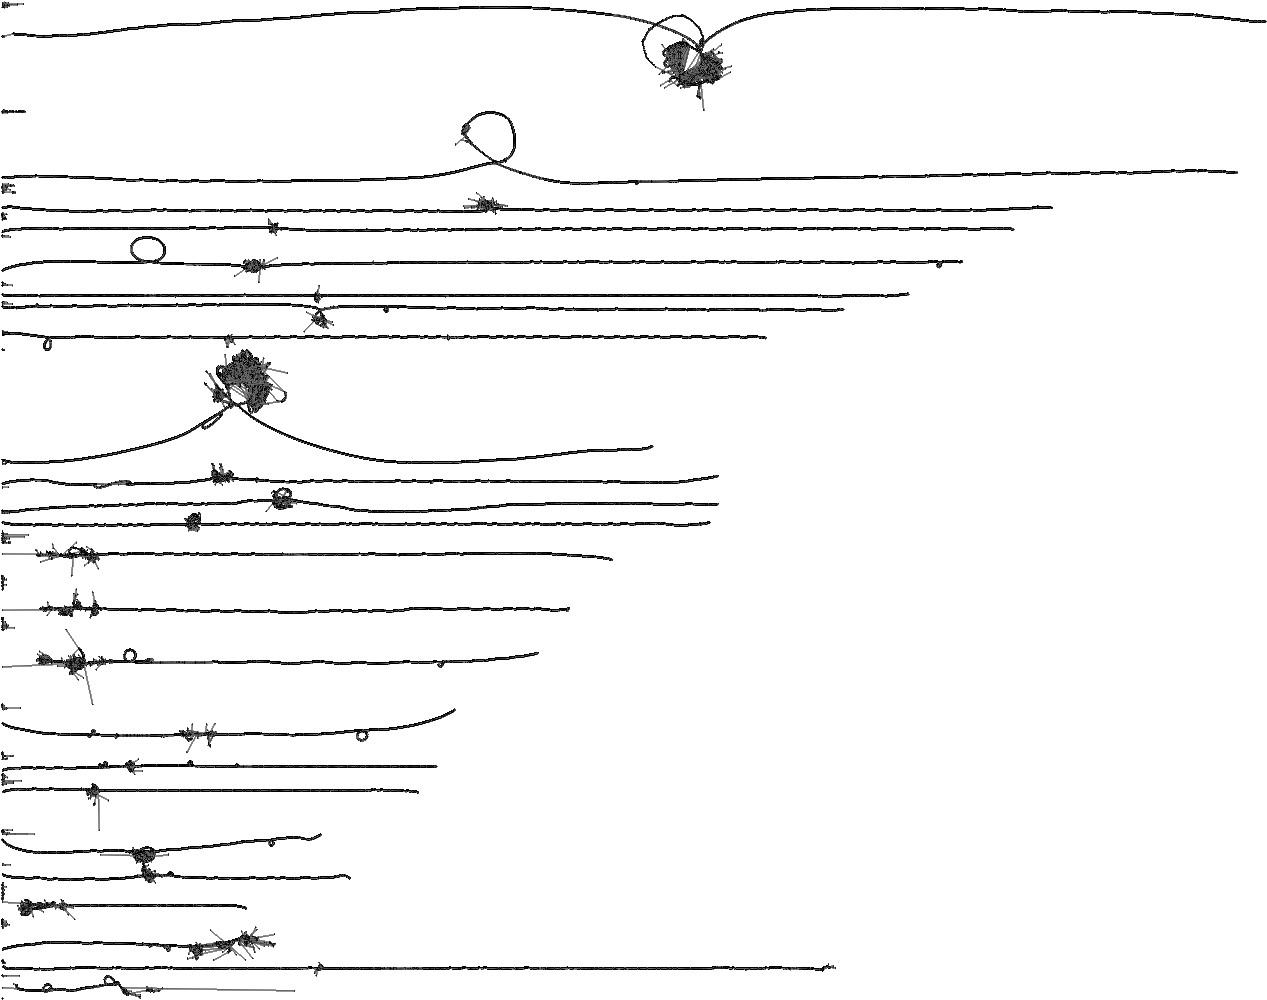
\includegraphics[width=1.0\linewidth]{fig/2D/2D_all_chroms.png}
		\label{fig:sfig1}
	\end{subfigure}
	\\
	\begin{subfigure}{1.0\textwidth}
		\centering
		\caption{}
		
\includegraphics[width=1.0\linewidth]{fig/2D/grch38.chr6.MHC_annotated.png}
		\label{fig:sfig2}
	\end{subfigure}
	\\
\begin{subfigure}{1.0\textwidth}
	\centering
	\caption{}
	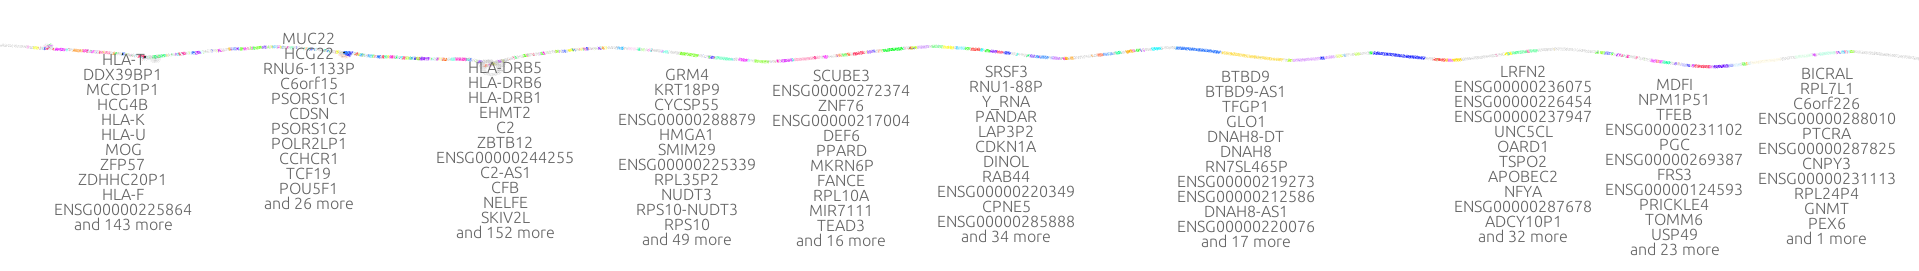
\includegraphics[width=1.0\linewidth]{fig/2D/grch38.chr6.MHC_genes_annotated.png}
	\label{fig:sfig3}
\end{subfigure}
	\\
\begin{subfigure}{1.0\textwidth}
	\centering
	\caption{}
	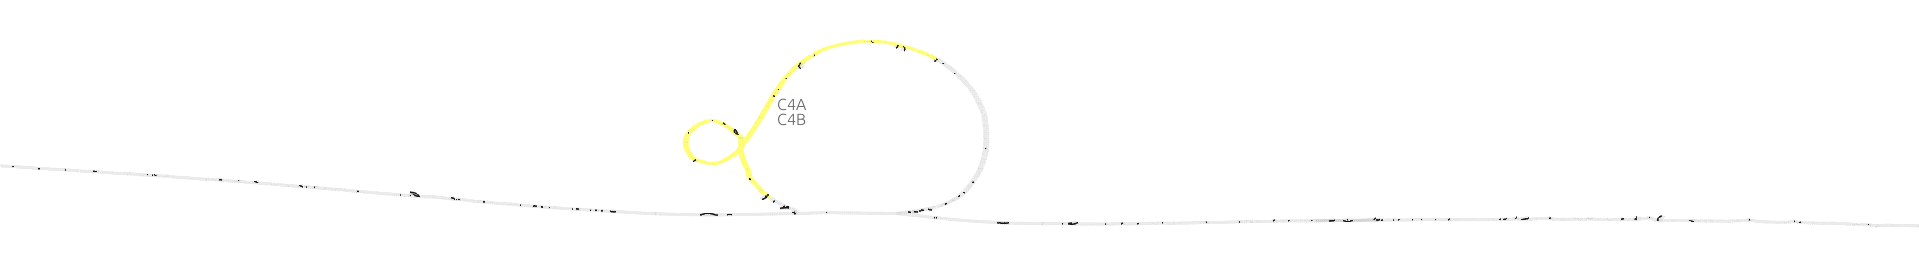
\includegraphics[width=1.0\linewidth]{fig/2D/grch38.chr6.C4_gene_annotated.png}
	\label{fig:sfig4}
\end{subfigure}	
	\caption{2D visualizations of all chromosomes of the Human Pangenome Resource Consortium (HPRC) Pangenome Graph Builder (PGGB) pangenome graph, chromosome 6, the major histocompatibility complex (MHC), and the complement component 4 (C4). \textbf{(a)} \textit{odgi draw} layout of the HPRC pangenome graph 90 haplotypes. Displayed are all 24 autosomes and the mitochondrial chromosome. \textbf{(b)} \textit{gfaestus} screenshot of the chromosome 6 layout highlighting the MHC. \textbf{(c)} \textit{gfaestus} screenshot of the MHC highlighting all genes in this region. \textbf{(d)} \textit{gfaestus} screenshot of the region around C4, specifically highlighting genes C4A and C4B.}
	\label{fig:2d_layouts}
\end{figure*}